% Options for packages loaded elsewhere
\PassOptionsToPackage{unicode}{hyperref}
\PassOptionsToPackage{hyphens}{url}
\documentclass[
  a4paper, twocolumn, DIV=calc]{scrartcl}
\usepackage[dvipsnames]{xcolor}
\usepackage{amsmath,amssymb}
\setcounter{secnumdepth}{-\maxdimen} % remove section numbering
\usepackage{iftex}
\ifPDFTeX
  \usepackage[T1]{fontenc}
  \usepackage[utf8]{inputenc}
  \usepackage{textcomp} % provide euro and other symbols
\else % if luatex or xetex
  \usepackage{unicode-math} % this also loads fontspec
  \usepackage[backend=biber,style=alphabetic]{biblatex}
  \addbibresource{references.bib}
  \defaultfontfeatures{Scale=MatchLowercase}
  \defaultfontfeatures[\rmfamily]{Ligatures=TeX,Scale=1}
\fi
\usepackage{tikz}
\usetikzlibrary{positioning, decorations.pathreplacing}
\usetikzlibrary{calc, decorations.pathreplacing}
\usetikzlibrary{arrows.meta, shapes.geometric}
\usepackage{lmodern}
\ifPDFTeX\else
  % xetex/luatex font selection
  \setmainfont[]{Libertinus Serif}
  \setsansfont[]{Libertinus Sans}
  \setmonofont[]{Fira Code}
  \setmathfont[]{Libertinus Math}
  \usepackage{minted}
\fi
% Use upquote if available, for straight quotes in verbatim environments
\IfFileExists{upquote.sty}{\usepackage{upquote}}{}
\IfFileExists{microtype.sty}{% use microtype if available
  \usepackage[]{microtype}
  \UseMicrotypeSet[protrusion]{basicmath} % disable protrusion for tt fonts
}{}
\makeatletter
\@ifundefined{KOMAClassName}{% if non-KOMA class
  \IfFileExists{parskip.sty}{%
    \usepackage{parskip}
  }{% else
    \setlength{\parindent}{0pt}
    \setlength{\parskip}{6pt plus 2pt minus 1pt}}
}{% if KOMA class
  \KOMAoptions{parskip=half}}
\makeatother
\setlength{\emergencystretch}{3em} % prevent overfull lines
\providecommand{\tightlist}{%
  \setlength{\itemsep}{0pt}\setlength{\parskip}{0pt}}
\usepackage{bookmark}
\IfFileExists{xurl.sty}{\usepackage{xurl}}{} % add URL line breaks if available
\urlstyle{same}
\hypersetup{
  pdftitle={Formal Verification of the LZ77 and LZ78 Compression Algorithms},
  pdfauthor={Alexander Shekhovtsov; Ozair Faizan; Clément Tsedri},
  hidelinks,
  colorlinks=true,
  citecolor=Lavender,
  urlcolor=MidnightBlue,
  pdfcreator={LaTeX via pandoc}}

%%%%%% I don't know if this is allowed... %%%%%% 
\RedeclareSectionCommand[
  beforeskip=0.5\baselineskip,
  afterskip=0.3\baselineskip
]{section}
\RedeclareSectionCommand[
  beforeskip=0.4\baselineskip,
  afterskip=0.2\baselineskip
]{subsection}
\RedeclareSectionCommand[
  beforeskip=0.3\baselineskip,
  afterskip=0.1\baselineskip
]{subsubsection}


\title{Formal Verification of the LZ77 and LZ78 Compression Algorithms}
\usepackage{etoolbox}
\makeatletter
\providecommand{\subtitle}[1]{% add subtitle to \maketitle
  \apptocmd{\@title}{\par {\large #1 \par}}{}{}
}
\makeatother
\subtitle{CS-428 project report}
\author{Alexander Shekhovtsov \and Clément Tsedri \and Ozair Faizan}
\date{2026-05-31}

\begin{document}
\maketitle

\section{Abstract}

Lempel-Ziv compression algorithms \cite{ZivLempel1977, ZivLempel1978} are the
backbone of
many widely used compression algorithms, including DEFLATE, gzip, and
zip. In this project, we modeled and formally proved the functional
correctness of both algorithms in Rocq, alongside upper bounds on their
worst-case compressed output lengths. Originally we proposed
verification of low-level C implementation using the Verified Software
Toolchain
\href{https://github.com/PrincetonUniversity/VST}{VST}, however,
verifying low-level memory operations and pointer arithmetic in VST is
excessively time-consuming even for simple array manipulations, leading
us to focus only on the high-level functional correctness.

\textbf{Keywords:} Formal verification, Lempel-Ziv, LZ77, LZ78,
functional correctness, data compression.

\section{Introduction}

Data compression is widely-used in day-to-day and security-sensitive
applications, yet its correctness often relies on manual testing rather
than formal verification.

\subsection{LZ77 Algorithm}

The LZ77 algorithm operates over a sliding window of
previously seen bytes. During compression, the algorithm scans the input
and, at each position, searches the window for the longest match to the
upcoming bytes. If a match of length at least 3 is found, it emits a
reference token \texttt{(length,\ offset)}, where offset is the distance
to the start of the match in the window. Otherwise, it emits a literal
token containing the current byte. These references are packed into two
bytes: 4 bits for the length and 12 bits for the offset. Therefore,
they are limited to the range \([3, 18]\) and \([3, 4098]\)
respectively, as a bias of +3 is used.

\begin{figure}[h]
    \centering
    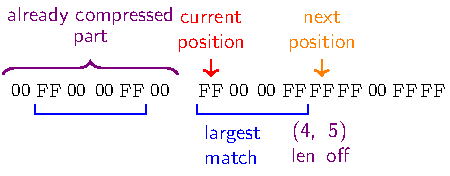
\includegraphics{figs/lz77.pdf}
    \caption{
      Illustration of LZ77 compression algorithm. The blue segment is the
      largest match in the window. It is of length 4 and with an offset of
      5 from the current position.
    }
    \label{fig:LZ77}
\end{figure}


\subsection{LZ78 Algorithm}

LZ78 takes a dictionary-based approach. It maintains an explicit
dictionary of previously seen bit sequences, starting with a single
empty entry. At each step, the algorithm finds the longest prefix of the
remaining input that already appears in the dictionary, then emits a
token \texttt{(index,\ next\_bit)} pointing to that dictionary entry
and the following bit. The concatenation of the matched prefix and the
new bit is then added to the dictionary.

\begin{figure}[h]
    \centering
    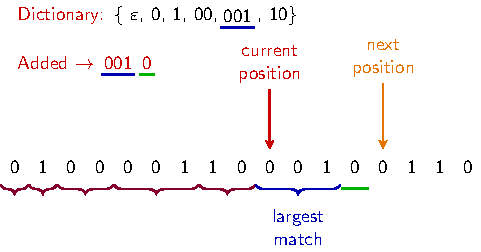
\includegraphics{figs/lz78.pdf}
    \caption{Illustration of LZ78 compression algorithm. The blue segment is the largest match with a word from dictionary. The string $0010$ is refered to as a new \textit{phrase}. Note that as a result of its work, the algorithm partitions the input string into distinct phrases (purple segments).}
    \label{fig:LZ78}
\end{figure}

\subsection{Problem Statement}

The goal of this project is to verify end-to-end correctness of the compression
algorithm by proving that decompression recovers the original data from the
compressed data. Additionally, provide an upper bound on the compressed output
size.

\section{Approach}

Compression proceeds in two passes, in the first pass, the input byte/bit
sequence is converted to a list of abstract tokens and in the second pass, the
token list is serialized to bytes/bits. Decompression reverses these steps. This
two-level design cleanly separates the compression logic from the byte/bit encoding
and simplifies the reasoning.

\subsection{LZ77 Implementation}
\subsubsection{Token Definition}
The first pass of LZ77 produces a list of \texttt{Token}s. A token is either a
literal byte or a back-reference.
\begin{minted}{coq}
Inductive Token :=
  | Lit (b: byte)
  | Ref (length offset: nat).
\end{minted}
A token is considered
\href{https://github.com/Jatana/LZ78FormalVerification/blob/2819b54b6eb88639461c4fd3504fbc2a87e8cbc0/lz77/LZ_Tokens.v#L11}{\emph{valid}}
if a reference token satisfies the constraints on \texttt{length} and
\texttt{offset}. A key
\href{https://github.com/Jatana/LZ78FormalVerification/blob/2819b54b6eb88639461c4fd3504fbc2a87e8cbc0/lz77/LZ.v#L39}{lemma}
is that compression produces valid tokens.

\subsubsection{Matching}
The matching module implements the sliding-window search.
\href{https://github.com/Jatana/LZ78FormalVerification/blob/2819b54b6eb88639461c4fd3504fbc2a87e8cbc0/lz77/LZ_Matching.v#L33}{\texttt{find\_largest\_match}}
find the largest match that satisfies the constraints on
\href{https://github.com/Jatana/LZ78FormalVerification/blob/2819b54b6eb88639461c4fd3504fbc2a87e8cbc0/lz77/LZ_Matching.v#L99}{\texttt{length}}
and \href{https://github.com/Jatana/LZ78FormalVerification/blob/2819b54b6eb88639461c4fd3504fbc2a87e8cbc0/lz77/LZ_Matching.v#L153}{\texttt{offset}}.
The key correctness lemma about matching is
\href{https://github.com/Jatana/LZ78FormalVerification/blob/2819b54b6eb88639461c4fd3504fbc2a87e8cbc0/lz77/LZ_Matching.v#L214}{\texttt{find\_largest\_match\_eq}}
which states that the slice of \texttt{before} at the reported offset byte-wise
equals the corresponding prefix of \texttt{after} of the reported length.

\subsubsection{Compression and Decompression}
The compression is defined by the auxiliary function
\href{https://github.com/Jatana/LZ78FormalVerification/blob/2819b54b6eb88639461c4fd3504fbc2a87e8cbc0/lz77/LZ.v#L7}
{\texttt{compress\_aux before after l}}, where \texttt{before} is the bytes
already processed, \texttt{after} is the remaining input, and \texttt{l} is a
skip counter that advances past the bytes already covered by the most recent
back-reference. When the skip counter is zero, it either emits a literal or a
back-reference and sets the skip counter to \texttt{length-1} to skip over the
matched bytes.
The decompression
\href{https://github.com/Jatana/LZ78FormalVerification/blob/2819b54b6eb88639461c4fd3504fbc2a87e8cbc0/lz77/LZ.v#L21}{\texttt{decompress\_aux acc token}}
mirrors the structure, a literal token appends its byte to \texttt{acc}, a reference token
copies \texttt{length} bytes from $\texttt{acc}[k; k+\texttt{length})$ where
$k=|\texttt{acc}|-\texttt{offset}$.

\subsubsection{Token Serialization}
The second pass serializes tokens to bytes. Each valid reference token is packed
into two bytes by
\href{https://github.com/Jatana/LZ78FormalVerification/blob/2819b54b6eb88639461c4fd3504fbc2a87e8cbc0/lz77/LZ_Tokens.v#L200}{\texttt{token\_to\_bytes}}.
The upper nibble of the first byte holds \texttt{length-3}, the lower nibble
holds the high byte of \texttt{offset-3}, and the second byte holds its low
byte.
A flag bit is required to distinguish between bytes encoding literals and bytes
encoding references, therefore,
\href{https://github.com/Jatana/LZ78FormalVerification/blob/2819b54b6eb88639461c4fd3504fbc2a87e8cbc0/lz77/LZ_Tokens.v#L218}{\texttt{tokens\_to\_bytes\_chunk}}
prepends a flag byte for the following 8 tokens encoding.
Finally,
\href{https://github.com/Jatana/LZ78FormalVerification/blob/2819b54b6eb88639461c4fd3504fbc2a87e8cbc0/lz77/LZ_Tokens.v#L245}{\texttt{tokens\_to\_bytes}}
recursively calls \texttt{tokens\_to\_bytes\_chunk} to serialize the token list.
Moreover, the inverses of these functions are also defined for decompression.

As a verification of a C implementation was expected, we needed to encode the length of
the original input, so that a large enough buffer could be allocated. Therefore,
a \href{https://github.com/Jatana/LZ78FormalVerification/blob/2819b54b6eb88639461c4fd3504fbc2a87e8cbc0/lz77/LZ_Tokens.v#L34}{variable-length
encoding} is prepended to the compressed bytes, however it is never actually
used by the decompression algorithm (since in Rocq we have access to the length of a list).


\subsection{LZ78 Implementation}
\subsubsection{Token Definition}
LZ78 operates over bits rather than bytes to simplify the upper bound theorem.
Again, the first pass produces a list of \texttt{Token}s.
\begin{minted}{coq}
Inductive Token :=
  | Tok  (index: nat) (phr : list bool) (next: bool)
  | Last (index: nat) (phr : list bool). 
\end{minted}
\texttt{Tok} carries the dictionary \texttt{index} of the matched prefix \texttt{phr},
and the following bit \texttt{next}. \texttt{Last} token may be used as the very
last token if the match exhausts the remaining input buffer. The phrases
\texttt{phr} are for proof purposes only (when converting tokens to bits, phr is not used).

\subsubsection{Dictionary and Matching}
The dictionary has type
\href{https://github.com/Jatana/LZ78FormalVerification/blob/2819b54b6eb88639461c4fd3504fbc2a87e8cbc0/lz78/LZ_Dict.v#L7}{\texttt{list (list bool)}},
initialised as
\href{https://github.com/Jatana/LZ78FormalVerification/blob/2819b54b6eb88639461c4fd3504fbc2a87e8cbc0/lz78/LZ_Dict.v#L8}{\texttt{empty\_dict := [[]]}}.
The function
\href{https://github.com/Jatana/LZ78FormalVerification/blob/2819b54b6eb88639461c4fd3504fbc2a87e8cbc0/lz78/LZ_Dict.v#L31}{\texttt{find\_largest\_prefix}}
scans the dictionary for the entry with the largest length that is a prefix of the
remaining input, returning its index and length.

\subsubsection{Compression and Decompression}
Both the compression and decompression algorithms are similar enough to LZ77 to
not require further detail.

\subsubsection{Token Serialization}
The second pass serializes tokens to bits. Each token's index is encoded with
\href{https://github.com/Jatana/LZ78FormalVerification/blob/2819b54b6eb88639461c4fd3504fbc2a87e8cbc0/lz78/LZ_Dict.v#L10}{\texttt{num\_bits\_for\_dict}} 
$ = \lceil \log_2|\texttt{dict}| \rceil$ bits.
The deserializer computes $|\texttt{dict}|$ by counting the number of tokens, as
each token equates to a dictionary entry.
Similar to LZ77, \href{https://github.com/Jatana/LZ78FormalVerification/blob/2819b54b6eb88639461c4fd3504fbc2a87e8cbc0/lz78/LZ_Tokens.v#L83}{\texttt{tokens\_to\_bits}}
and its left-inverse \href{https://github.com/Jatana/LZ78FormalVerification/blob/2819b54b6eb88639461c4fd3504fbc2a87e8cbc0/lz78/LZ_Tokens.v#L103}{\texttt{bits\_to\_tokens}}
are defined.

\section{Results}

\subsection{LZ77 Correctness}

The correctness theorem is proved in two steps. In the first step
\begin{minted}{coq}
Theorem compress_decompress_correctness_aux:
  forall n bef aft, length aft <= n ->
    decompress_aux bef (compress_aux bef aft 0)
      = bef ++ aft.
\end{minted}
is proved by strong induction on $n$ (the length of \texttt{aft}).
The \href{https://github.com/Jatana/LZ78FormalVerification/blob/2819b54b6eb88639461c4fd3504fbc2a87e8cbc0/lz77/LZ.v#L95}{proof}
proceeds by case analysis on whether a match is found. In the literal
case the goal follows immediately. In the reference case, several lemmas about
the \texttt{slice} function and the correctness lemmas about
\texttt{find\_largest\_match} are used.
\href{https://github.com/Jatana/LZ78FormalVerification/blob/2819b54b6eb88639461c4fd3504fbc2a87e8cbc0/lz77/LZ.v#L58}{\texttt{compress\_rolls}}
which shows that advancing the skip counter is equivalent to prepending the
skipped bytes to \texttt{before} and compressing the remainder, is a key lemma.

The second step is to prove the full round-trip:
\begin{minted}{coq}
Theorem compress_to_bytes_correctness:
  forall s,
    decompress_from_bytes
      (compress_to_bytes s) = s.
\end{minted}
Since the compression logic is separated from the serialization logic, we
\href{https://github.com/Jatana/LZ78FormalVerification/blob/2819b54b6eb88639461c4fd3504fbc2a87e8cbc0/lz77/LZ_Tokens.v#L683}{proved} that
\begin{minted}{coq}
Theorem tokens_to_bytes_to_tokens_correctness:
  forall t, Forall valid_token t ->
    bytes_to_tokens (tokens_to_bytes t) = t.
\end{minted}
As \texttt{compress\_to\_bytes} and \texttt{decompress\_from\_bytes} are defined
as $\texttt{tokens\_to\_bytes} \circ \texttt{compress}$  and
$\texttt{decompress} \circ \texttt{bytes\_to\_tokens}$ (ignoring the length
encoding), the proof of the above theorem follows immediately from the two
correctness lemmas.


\subsection{LZ77 Upper Bound}
The worst case of LZ77 occurs when no match is ever found during the compression
process and every byte is emitted as a literal. Since the encoding of each literal 
requires an additional flag bit, the worst case upper bound is (ignoring length
encoding) given by 
$$ |\texttt{compress\_to\_bytes } s| \leqslant \left\lceil\frac{9 |s|}{8} \right\rceil .$$
To prove this bound we first assign each token a weight: 1 for literals and 3 for references.
The weight represents the smallest prefix each token can consume.
The \href{https://github.com/Jatana/LZ78FormalVerification/blob/2819b54b6eb88639461c4fd3504fbc2a87e8cbc0/lz77/LZ_Tokens.v#L727}{\texttt{tokens\_to\_bytes\_bounded\_by\_weight}}
and \href{https://github.com/Jatana/LZ78FormalVerification/blob/2819b54b6eb88639461c4fd3504fbc2a87e8cbc0/lz77/LZ.v#L196}{\texttt{compress\_weight\_upper\_bound}}
are used to prove the chain of inequalities
$$ |\texttt{compress\_to\_bytes } s| \leqslant
\left\lceil \frac{9\sum_i\texttt{weight }t_i}{8} \right\rceil \leqslant 
\left\lceil \frac{9|s|}{8} \right\rceil .$$

\subsection{LZ78 Correctness}
The correctness proofs are similar enough to LZ77 to not require further detail.

% \subsection{LZ78 Upper Bounds}
% We have formally proved that the length of the compressed string is at most $|s| + 21 \cdot |s|/\log_2 |s|$:
% 
% \begin{minted}{coq}
% Theorem compress_to_bits_bound: forall s n k,
% n = length (compress s) -> 10 <= Nat.log2 n ->
% k = length s -> 12 <= Nat.log2 k ->
% length (compress_to_bits s) <= k + 21*k / Nat.log2 k.
% \end{minted}
% 
% The proof of the theorem follows from two inequalities.
% 
% (1) The upper bound on the compressed string in terms of \textit{length tokens}:
% \begin{minted}{coq}
% Lemma tokens_to_bits'_length_bound:
% forall tokens dict_size max_dict_size,
% dict_size + length tokens <= max_dict_size ->
% length (tokens_to_bits' dict_size tokens)
% <= length tokens * (num_bits_for_dict max_dict_size+1).
% \end{minted}
% where 
% 
% \begin{minted}{coq}
% Definition num_bits_for_dict (dict_size: nat) :=
% if dict_size <=? 1 then 1
% else (Nat.log2 (dict_size - 1)) + 1.
% \end{minted}
% 
% (2) The lower bound on the initial string $s$ in terms of \textit{length tokens}:
% 
% \begin{minted}{coq}
% Lemma compress_bound: forall s tokens,
% compress s = tokens ->
% length s >= (length tokens - 1)
%     * (Nat.log2 (length tokens - 1) - 2).
% \end{minted}
% 
% The first inequality is relatively straightforward since the size of the dictionary is bounded by \textit{length tokens}, and for each token we spend logarithmically many bits to encode its position in the dictionary plus one bit to encode \textit{next\_bit}. The second inequality is proved using the fact that the phrases that the initial string $s$ is partitioned into are distinct (disregarding the last phrase). Formally, by induction on fuel we prove
% 
% \begin{minted}{coq}
% Lemma compress'_phrases_differ:
% forall fuel dict s tokens prev_tokens,
% length s <= fuel ->
% compress' fuel dict s = tokens ->
% agreement dict prev_tokens ->
% nth_error dict 0 = Some [] ->
% phrases_differ prev_tokens tokens
%     /\ phrases_differ_one tokens.
% \end{minted}
% 
% where \textit{agreement} certifies that all tokens from \textit{prev\_tokens} are in the dictionary, and \textit{phrases\_differ} certifies that the phrases corresponding to tokens are distinct. Using the knowledge that the phrases are distinct, it suffices to prove that if $p_1 + p_2 + \ldots + p_m = s$ holds for a string $s$ and $p_1, p_2, \ldots, p_m$ are pairwise different, then $|s| \geq m \cdot (\log_2 m - 2)$. Let us show how to prove it in the next section.
% 
% \subsubsection{Proof of Combinatorial Theorem}
% 
% Let us prove 
% 
% \begin{minted}{coq}
% Lemma corr_lb : forall l,
% different l ->
% list_sum (map (@length (bool)) l) >= (length l)
%         *(Nat.log2(length l) - 2).
% \end{minted}
% 
% Here we define different $l$ as $l_i \neq l_j$ for $i \neq j$:
% \begin{minted}{coq}
% Definition different (l : list (list bool))
%     := forall i j a b,
% i <> j -> nth_error l i = Some a ->
% nth_error l j = Some b -> a <> b.
% \end{minted}
% 
% To prove the theorem we decompose it into several lemmas. The first lemma states that there can be at most $2^{n+1} - 1$ distinct strings of length $\leq n$.
% 
% \begin{minted}{coq}
% Lemma diff_strings_leq_n : forall n l,
% different l ->
% length(filter(equal_or_less_len_n n) l)
%     <= 2^(n+1)-1.
% \end{minted}
% 
% To prove \textit{diff\_strings\_leq\_n}, we first prove the upper bound for the number of strings of length exactly $n$. The proof is by induction on $n$. We partition all strings into ones that start with $0$ and into ones that start with $1$. We apply induction hypothesis to bound their number by $2^{n-1}$, giving $2 \cdot 2^{n-1}$ bound on the number of initial strings.
% 
% Now, by using \textit{diff\_strings\_leq\_n} and properties of filter function, we establish that there are many strings of length at least $n$:
% \begin{minted}{coq}
% Lemma diff_lb : forall n l,
% different l ->
% length (filter (equal_or_greater_len_n n) l)
%     >= length l + 1 - 2^n.
% \end{minted}
% 
% At this point, let us express the sum of lengths of all strings $\sum_i |l_i|$ as the sum over an indicator
%     $$\sum_i \sum_k I(|l_i| \geq k).$$
% 
% Our goal is to exchange the summations. We have proven a general statement that summations can be exchanged by induction on $n$ and $m$:
% 
% \begin{minted}{coq}
% Lemma sum_row_sum_col :
% forall (n m : nat) (f : nat -> nat -> nat),
% sum_over (fun i => sum_over (f i) m) n
% = sum_over (fun j => sum_over (fun x => f x j) n) m.
% \end{minted}
% 
% Here $\textit{sum\_over}(g, m) = g(0) + g(1) + \ldots + g(m - 1)$. Using \textit{sum\_row\_sum\_col} and \textit{diff\_lb}, we get the desired bound
% 
% \begin{align*}
% \sum_i \sum_k I(|l_i| \geq k) &=
% \sum_k \sum_i I(|l_i| \geq k) \geq \\
% \sum_{k \leq \log_2 |l|} \left(|l| + 1 - 2^k \right) &\geq
% |l| \cdot (\log_2 |l| - 2).
% \end{align*}

\subsection{LZ78 Upper Bound}
We \href{https://github.com/Jatana/LZ78FormalVerification/blob/2819b54b6eb88639461c4fd3504fbc2a87e8cbc0/lz78/LZ.v#L1469}{proved}
an asymptotic upper bound on the compressed size:
$|\texttt{compress\_to\_bits } s| \leqslant |s| + o(|s|) = |s| + 21|s|/\log_2|s|.$
\begin{minted}{coq}
Theorem compress_to_bits_bound: forall s n k,
  n = length (compress s) ->
  k = length s ->
  10 <= Nat.log2 n ->
  12 <= Nat.log2 k ->
  length (compress_to_bits s)
    <= k + 21 * k / Nat.log2 k.
\end{minted}

The proof uses two inequalities. The
\href{https://github.com/Jatana/LZ78FormalVerification/blob/2819b54b6eb88639461c4fd3504fbc2a87e8cbc0/lz78/LZ.v#L184}{first}
bounds the bit length in 
terms of the number of tokens, since each token at dictionary size $d$
requires $\lceil \log_2 d\rceil$ bits.
The \href{https://github.com/Jatana/LZ78FormalVerification/blob/2819b54b6eb88639461c4fd3504fbc2a87e8cbc0/lz78/LZ.v#L1124C9-L1124C41}{\texttt{second}}
is a lower bound on $|s| \geqslant m \cdot (\log_2 m - 2)$ in terms of the
number of tokens $m$. The theorem is proved using the fact that $s = p_1 + p_2 +
\ldots + p_m$ is
\href{https://github.com/Jatana/LZ78FormalVerification/blob/2819b54b6eb88639461c4fd3504fbc2a87e8cbc0/lz78/LZ.v#L256}{partitioned into distinct phrases}.
We establish the following sequence of inequalities that allows us to lower
bound $|s|$.
\begin{align*}
|s| &= \sum_{i=1}^m |p_i|
        \overset{(1)}{\geqslant} \sum_{i=1}^m\sum_{k=1}^{\log_2 m} I(|p_i| \geqslant k)
        \overset{(2)}{=} \sum_{k=1}^{\log_2 m} \sum_{i=1}^m I(|p_i| \geqslant k) \\
    &\overset{(3)}{\geqslant} \sum_{1 \leqslant k \leqslant \log_2 m} (m + 1 - 2^k)
     \overset{(4)}{\geqslant} m \cdot (\log_2 m - 2)
\end{align*}

The bound (1)
(\href{https://github.com/Jatana/LZ78FormalVerification/blob/2819b54b6eb88639461c4fd3504fbc2a87e8cbc0/lz78/LZ.v#L903}{\texttt{sum\_over\_list\_sum}})
is established using lemma
\href{https://github.com/Jatana/LZ78FormalVerification/blob/2819b54b6eb88639461c4fd3504fbc2a87e8cbc0/lz78/LZ.v#L883C9-L883C27}{\texttt{sum\_over\_indicator}}
that allows to express a number as the sum of indicators. We prove that two
summations can be swapped in
\href{https://github.com/Jatana/LZ78FormalVerification/blob/2819b54b6eb88639461c4fd3504fbc2a87e8cbc0/lz78/LZ.v#L833}{\texttt{sum\_row\_sum\_col}}
(2). In
\href{https://github.com/Jatana/LZ78FormalVerification/blob/2819b54b6eb88639461c4fd3504fbc2a87e8cbc0/lz78/LZ.v#L736}{\texttt{distinct\_length\_ge\_n\_lower\_bound}},
we prove that at least $m - 2^{k+1} + 1$ strings from $p_1, \ldots, p_m$ have
length at least $k$, allowing us to conclude (3).
Finally,
\href{https://github.com/Jatana/LZ78FormalVerification/blob/2819b54b6eb88639461c4fd3504fbc2a87e8cbc0/lz78/LZ.v#L1046}{\texttt{sum\_over\_log2\_lower\_bound}}
proves (4).
Using the resulting \href{https://github.com/Jatana/LZ78FormalVerification/blob/2819b54b6eb88639461c4fd3504fbc2a87e8cbc0/lz78/LZ.v#L1077}{lower bound} and some
\href{https://github.com/Jatana/LZ78FormalVerification/blob/2819b54b6eb88639461c4fd3504fbc2a87e8cbc0/lz78/LZ.v#L1383}{asymptotic bounds},
the \href{https://github.com/Jatana/LZ78FormalVerification/blob/2819b54b6eb88639461c4fd3504fbc2a87e8cbc0/lz78/LZ.v#L1469}{upper bound} is established.


\subsection{Limitations}
Our original proposal included verification of a C implementation using
VST. We were unable to complete this, for several reasons mainly related to VST
itself. VST is known to be labor-intensive where simple array manipulations may
require substantial efforts to prove. This is well-documented by Andrew Appel
\cite[16]{VSTSHA} who participated in the creation of the framework.
Furthermore, our two pass approach simplified the formalization, however C
implementations perform a single pass writing directly into the output byte
buffer.
We also attempted to write recursive C functions to match the Rocq fixpoints,
but this along with other attempts at
\href{https://github.com/Jatana/LZ78FormalVerification/blob/a4188da3bfc59da321dffea4d105660a756dabc1/lz77/verif_LZC.v}{VST proofs}
were not too successful. 


\section{Timeline}
The proofs of LZ77 correctness and upper bound were done a week earlier than
planned.
Then, we had 3 weeks (originally 2) to prove the correctness of our C
implementation, however, after dedicating two weeks to VST without any
progress, we made the decision to pivot our scope. We reallocated our remaining
schedule to formally model, prove the correctness, and an asymptotic upper bound
of the LZ78 algorithm instead.

At the start of each major step (new theorem/new algorithm) we laid out the
functions to implement and lemmas to prove. The proofs were started while
pair coding, and then finalized separately.
LZ77 and LZ78 upper bounds were done by Alexander Shekhovtsov.
LZ78 simple upper bound was done by Clément Tsedri.
LZ77 and LZ78 serialization, LZ78 correctness and the asymptotic bound section
were done by Ozair Faizan.
All other lemmas and theorems had roughly equal contribution. 


\section{Related work}

Our project closely aligns with existing data compression verification efforts,
most notably \href{https://github.com/kim-em/lean-zip}{lean-zip} which is an
implementation and verification of the LZ77 algorithm within the DEFLATE
standard written in Lean 4. Our work differs by targeting both LZ77 and LZ78 in
Rocq, and providing concrete upper bounds on compressed size.

There is a
\href{https://github.com/PrincetonUniversity/VST/blob/master/doc/catalog-of-examples.md}{catalog
of examples} of VST-based verifications, most notably,
\cite{VSTSHA}.
These projects confirm the significant cost of VST-based verification,
consistent with our experience.

\section{Future work: Asymptotic Optimality}
Lempel and Ziv \cite{ZivLempel1978} proved that LZ78 algorithm is at least as efficient as any finite state (FS) compressor. More precisely, for any infinite string $s \in \{0, 1\}^{\mathbb{N}}$ and any FS compressor $C$ with $q$ states, the upper limit $\lim \sup_n |\textit{LZ78}(s[1:n])|/n$ is bounded above by the lower limit $\lim \inf_n |C(s[1:n])|/n$.

To prove the theorem authors use the fact that LZ78 compressor partitions the initial string into distinct phrases $p_1 + p_2 + \ldots + p_m = s$. They show that a finite state compressor $C$ should spend at least $m \cdot (\log_2 m - O(1))$ bits to compress $s$ and that the length of the initial string is at least $m \cdot (\log_2 m - 2)$, which we have proved in this work. Therefore, to complete the proof of the asymptotic optimality theorem, it remains to only prove the former result. This allows to show that the length of the compressed string is not only not larger than the length of the initial string, but also can be significantly smaller if there is a FS compressor that can greatly reduce its length.

\section{Conclusion}

We have presented proofs for the correctness of our implementation of LZ77 and
LZ78 compression algorithms. We additionally proved upper bounds on
compressed sizes.

The formalization demonstrates that a two-pass architecture (compression to
tokens, then token serialization) is well-suited for formal verification as it
allows independent proofs at each level.

Our experience with VST suggests that verifying a low-level C
implementation of LZ77 is feasible but requires substantially more
effort than the functional formalization.

This work provides a solid, foundation for Lempel-Ziv compression that
can serve as a basis for further verification of compression-related
software, including C implementations, streaming variants, and
higher-level algorithms built on the LZ family.

\section{AI use disclosure}

\begin{itemize}
\tightlist
\item
  Alexander Shekhovtsov
  \begin{itemize}
  \tightlist
  \item
    Used AI assistants to understand technical details of Verified Software Toolchain. 
    \item Used AI to help prove simple technical lemmas.
  \item 
    Used AI to generate tikz latex diagrams.
  \end{itemize}
\item
  Ozair Faizan
  \begin{itemize}
  \tightlist
  \item
    The LLMs are capable of proving some simple lemmas, however, for
    more challenging proofs they fails.
  \item
    Nevertheless, they were quite helpful for pen and paper proofs and
    brainstorming ideas.
  \end{itemize}
\item
  Clément Tsedri
  \begin{itemize}
  \tightlist
  \item
    ChatGPT is useful for small proofs or some formalisation details, 
    however they are not yet able to output correct proofs for more 
    challenging theorems outright
  \end{itemize}
\end{itemize}

\printbibliography

\end{document}
